\chapter{System topology}
利用热力学原理进行定性分析。提炼出创新点。
\section{System topology design}
\subsection{Basic systems}

The objective of this research is to research the equipment of solar thermal power generation system, to propose, develop and optimize a solar thermal cascade system depending on the advantages and disadvantages of the solar thermal power generation systems. 
The research is based on the national cooperation project "Collaborative research on key technologies to produce electricity by cascade utilization solar thermal energy" as the background. 
There are three kinds of mature technologies been applied commercially -- parabolic trough, parabolic dish and solar tower. 
Considering the future deployment of solar cascade demo system, two solar thermal technologies, parabolic trough and parabolic dish, are chosen as the basic systems for the design of cascade solar thermal power system. For the cascade utilization of the high temperature of the parabolic receiver, air (or nitrogen) is used as the HTF to transfer the heat collected.
Figure~\ref{fig:PTPD} shows the schematic diagrams of a parabolic trough system and a parabolic dish system.

\begin{figure}[!ht]
\centering
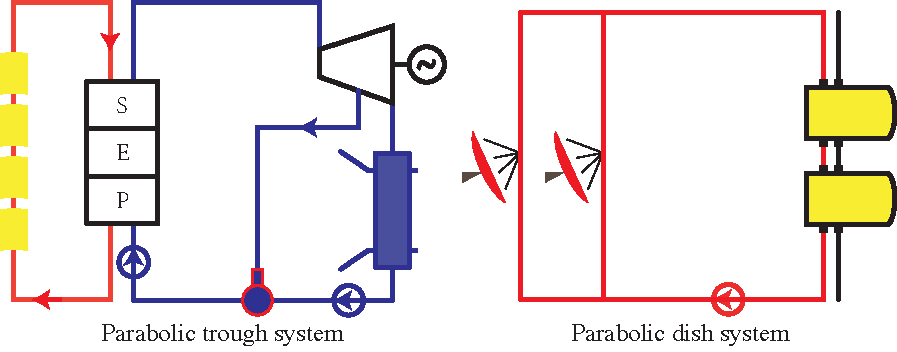
\includegraphics[width=0.8\textwidth]{fig/PTPD.pdf}
\caption{Schematic diagrams of a parabolic trough system and a parabolic dish system}\label{fig:PTPD}
\end{figure}

With different considerations (such as combination of different systems, water Rankine cycle or ORC, connection types of collectors, etc) of the cascade system topology, multiple combination topologies may be used for cascade systems. To get the most suitable system topology, these considerations will be analyzed in the following sections. 

\subsection{Solar chimney}
Solar chimney, also known as solar updraft tower, directly (without concentration) uses the sun's heat to generate power. It uses solar radiation to increase the internal air temperature to form a flow to the chimney located at the middle of the roof. Fig.~\ref{fig:SolarChimney} shows the schematic of a typical solar chimney power plant. In this plant, air is heat by the green house effect under the translucent roof. As the roof is open at its periphery, air flows into the plant due to different density distribution. Hot air flows into the chimney because of buoyancy. An electricity-generating turbine is set in the path of the air current to convert the kinetic energy of the flowing air into electricity.

\begin{figure}[!ht]
\centering 
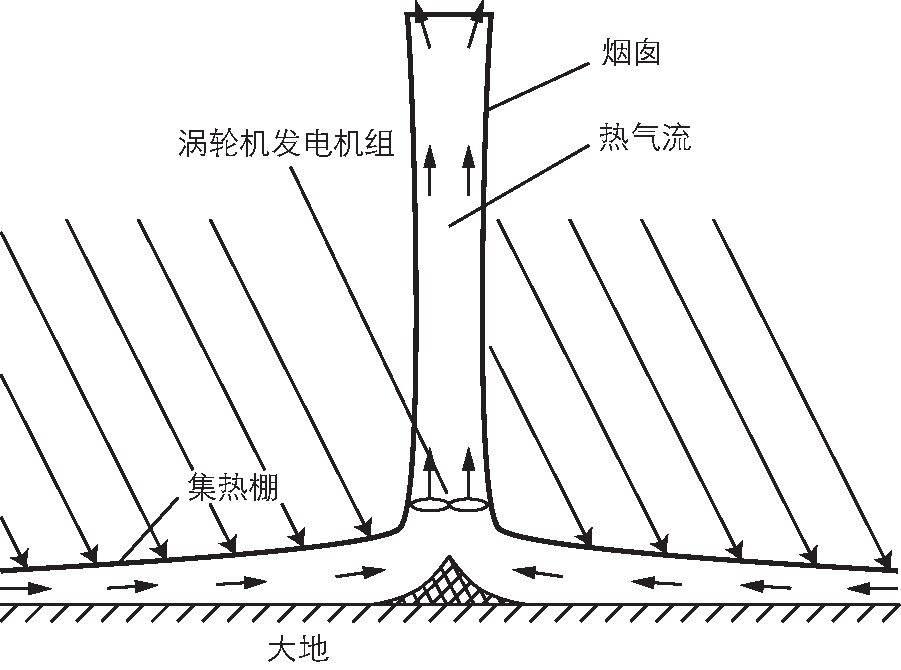
\includegraphics[width=0.7\textwidth]{fig/SolarChimney}
\caption{Schematic diagram of a solar chimney power plant}\label{fig:SolarChimney}
\end{figure}

The solar chimney can use the low temperature (low grade energy) for power generation. So the combination of parabolic trough system and solar chimney is considered an effective way for energy cascade utilization. In the combined system, the condenser in the Rankine cycle is air cooled. The fan blows the hot air that has cooled the condenser into the solar chimney power plant from its periphery. 



\section{System topology selection}
各种拓扑结构分析

